\documentclass[border=5pt]{standalone}
\usepackage{amsmath}
\usepackage{tikz}

% Macro replicated from main.tex
\newcommand{\Qmax}{Q_{\max}}

\begin{document}
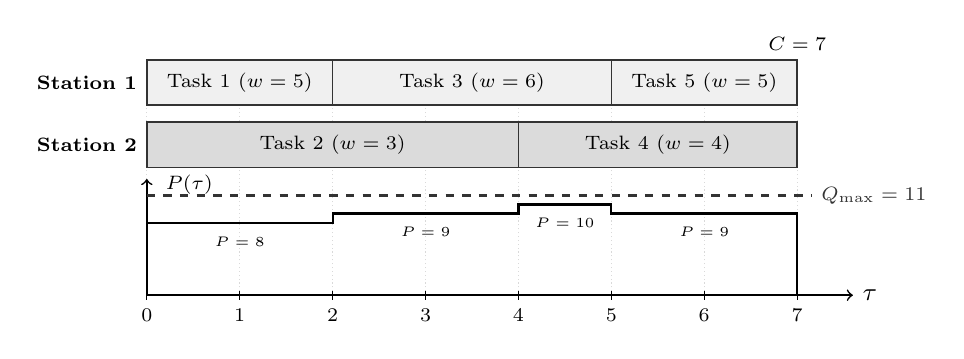
\begin{tikzpicture}[x=1.18cm,y=0.72cm,font=\small]
  % Shared time grid and axis
  \foreach \x in {0,...,7}{
    \draw[gray!30,densely dotted] (\x,0)--(\x,4.15);
    \draw (\x,0.08)--(\x,-0.08) node[below,font=\scriptsize]{\x};
  }
  \draw[->,semithick] (0,0)--(7.6,0) node[right]{$\tau$};
  
  % Station labels
  \node[left,font=\scriptsize\bfseries] at (0,3.75){Station 1};
  \node[left,font=\scriptsize\bfseries] at (0,2.65){Station 2};
  
  % Station 1 tasks (light gray fill, dark border)
  \filldraw[fill=gray!12,draw=black!80,semithick]
    (0,3.35) rectangle (2,4.15) node[midway,font=\scriptsize]{Task 1 ($w=5$)};
  \filldraw[fill=gray!12,draw=black!80,semithick]
    (2,3.35) rectangle (5,4.15) node[midway,font=\scriptsize]{Task 3 ($w=6$)};
  \filldraw[fill=gray!12,draw=black!80,semithick]
    (5,3.35) rectangle (7,4.15) node[midway,font=\scriptsize]{Task 5 ($w=5$)};
    
  % Station 2 tasks (pattern/medium gray fill, dark border)
  \filldraw[fill=gray!28,draw=black!80,semithick]
    (0,2.25) rectangle (4,3.05) node[midway,font=\scriptsize]{Task 2 ($w=3$)};
  \filldraw[fill=gray!28,draw=black!80,semithick]
    (4,2.25) rectangle (7,3.05) node[midway,font=\scriptsize]{Task 4 ($w=4$)};

  % Power profile axis
  \draw[->,semithick] (0,0)--(0,2.05);
  \node[anchor=west,font=\scriptsize\bfseries] at (0.10,1.95) {$P(\tau)$};
  
  % Cap line (dark dashed)
  \draw[black!80,dashed,thick]
    (0,1.76)--(7.15,1.76) node[right,font=\scriptsize\bfseries]{$\Qmax=11$};
    
  % Profile curve (solid black line)
  \draw[thick,black]
    (0,1.28)--(2,1.28)--(2,1.44)--(4,1.44)--(4,1.60)%
    --(5,1.60)--(5,1.44)--(7,1.44)--(7,0);
    
  % Power annotations below profile step segments
  \node[below=1.5pt,font=\tiny\bfseries] at (1,1.28){$P=8$};
  \node[below=1.5pt,font=\tiny\bfseries] at (3,1.44){$P=9$};
  \node[below=1.5pt,font=\tiny\bfseries] at (4.5,1.60){$P=10$};
  \node[below=1.5pt,font=\tiny\bfseries] at (6,1.44){$P=9$};
  
  \node[above,font=\scriptsize\bfseries] at (7,4.15){$C=7$};
\end{tikzpicture}
\end{document}
